\chapter{Fazit}
Ziel dieser Arbeit ist die Konzeption einer Software, welche zu übersetzende und übersetzte Strings der Texte eines Movelets automatisiert verarbeitet.
\par
Im Folgenden wird das im Zuge dieser Arbeit entstandene Konzept eines Lokalisierungstools vorgestellt. Um die Verwendung des Lokalisierungstools zu ermöglichen werden zu übersetzende Strings vom Nutzer ausgezeichnet. Zu diesem Zweck wird \ac{ITS} und die an \mbox{\textit{GNU gettext}} angelehnte Auszeichnung $\_()$ verwendet. Das Lokalisierungstool nutzt die Auszeichnung um zu übersetzende von nicht zu übersetzenden Strings zu unterscheiden. Infolgedessen extrahiert das Lokalisierungstool die ausgezeichneten Strings und erstellt \ac{XLIFF} Dateien. Die extrahierten Strings werden in den \mbox{\textit{source}} Elementen der \ac{XLIFF} Dateien gespeichert. \ac{XLIFF} wird als Schnittstelle zu externer Software verwendet.
In der Konsequenz kann dieses Format ohne Kompatibilitätsprobleme von in- und/oder externen Übersetzern und deren Software übersetzt werden. Die übersetzten Strings werden in den \mbox{\textit{source}} Elementen zugehörigen \mbox{\textit{target}} Elementen der \ac{XLIFF} Dateien gespeichert. Aus diesem Grund enthalten die \mbox{\textit{source}} Elemente die zu übersetzenden und die \mbox{\textit{target}} Elemente die zugehörigen übersetzten Strings. Aufgrund der Extraktion stimmt der Inhalt eines \mbox{\textit{source}} Elements mit einem ausgezeichneten String des Quelltexts des Movelets überein. Folglich wird durch das Ersetzen der ausgezeichneten Strings durch die Strings in den zugehörigen \mbox{\textit{target}} Elementen eine übersetzte Version des Quelltexts erzeugt. Zu diesem Zweck werden nicht die Strings im Originalquelltext ersetzt, stattdessen wird eine Kopie erzeugt, in welcher die Ersetzung erfolgt. Resultierend daraus fungiert der Originalquelltext als Vorlage, aus welcher beliebig viele übersetzte Versionen erzeugt werden können. 
\par
In Kapitel \ref{chp:version} wurde erarbeitet, dass dieses Lokalisierungstool keine Versionsverwaltung implementiert. Es ist jedoch empfehlenswert  Software zur Versionsverwaltung einzusetzen.
\par
Zum Zweck des besseren Verständnisses ist die Funktion des Lokalisierungstools in Abbildung \ref{fig:zsm} veranschaulicht. Die rote Linie zwischen Movelet-Vorlage und \ac{XLIFF} Datei stellt die Extraktion der zu übersetzenden Strings dar. Die Linien zwischen Übersetzer und \ac{XLIFF} Datei stellen den Vorgang der Übersetzung dar und die grüne Linie zwischen \ac{XLIFF} Datei und dem lokalisierten Movelet-EN stellt das Ersetzen der zu übersetzenden Strings in der Vorlage durch die übersetzten Strings dar.
\begin{figure}
	\centering
	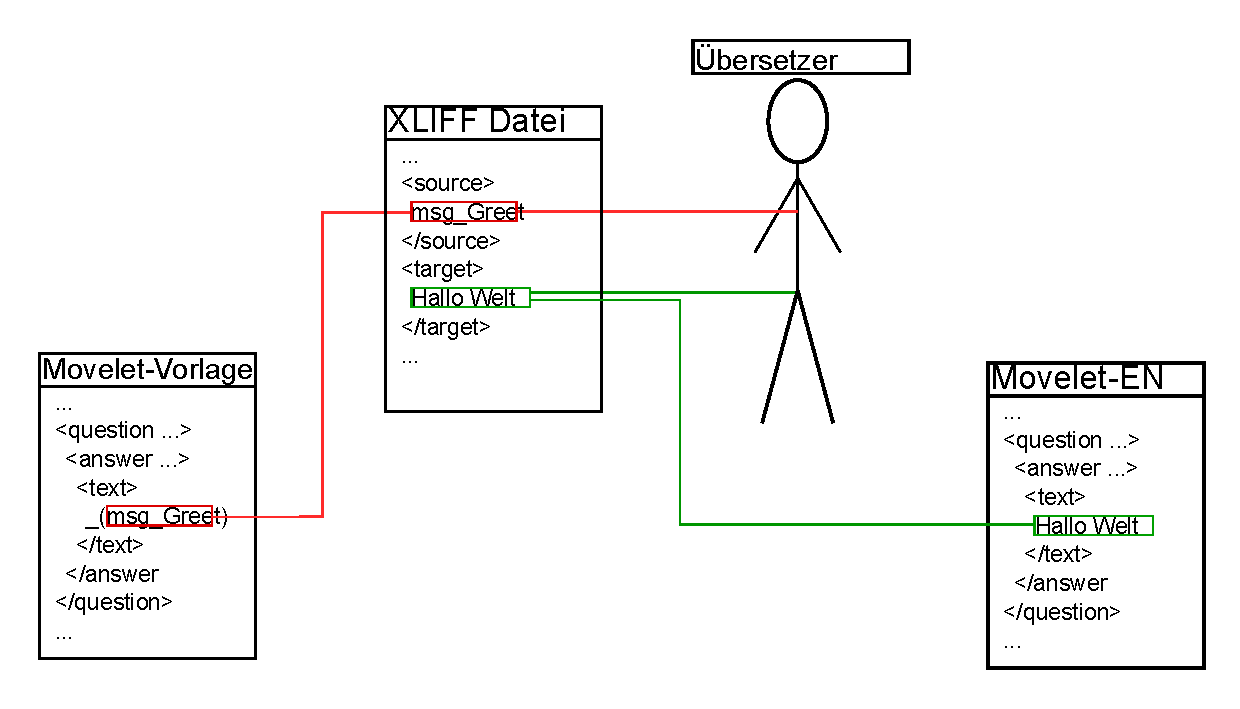
\includegraphics[width=1\textwidth]{img/zusammenfassung.pdf}
	\caption{Darstellung der Arbeitsschritte des Lokalisierungstools}
	\label{fig:zsm}
\end{figure}
\par
Das erarbeitete Lokalisierungstool greift bestehende Konzepte auf. Zu diesen Konzepten zählt die Auszeichnung von zu übersetzenden Strings, \ac{ITS}, \ac{XLIFF} und das Verwenden des Namens als Bezeichner. Die Auszeichnung von zu übersetzenden Strings, um diese von anderen Strings zu unterscheiden, wird von verschiedenen Lokalisierungstools verwendet. \ac{XLIFF} wurde von \ac{OASIS} für den Austausch von Daten der Lokalisierung entwickelt. Den Namen als Bezeichner zu verwenden ist ein grundlegendes Konzept der Bezeichnung.
\par
Das Alleinstellungsmerkmal des erarbeiteten Lokalisierungstools ist seine Einsatzmöglichkeit und Anpassung im Kontext von Movelets. Daher ist es die erste Software, die zum Zweck der Lokalisierung von Movelets eingesetzt werden kann. Aufgrund dessen hat dieses Lokalisierungstool das Potential den Prozess der Lokalisierung von Movelets zu revolutionieren.